\documentclass[11pt,a4paper]{article}
\usepackage[margin=2.4cm]{geometry}
\usepackage{graphicx}
\usepackage{amsmath}
\usepackage{amssymb}
\usepackage{booktabs}
\usepackage{multirow}
\usepackage[hidelinks]{hyperref}
\usepackage{xcolor}
\usepackage{setspace}
\graphicspath{{./}}
% pack floats with text instead of sparse float pages
\renewcommand{\topfraction}{0.9}
\renewcommand{\bottomfraction}{0.7}
\renewcommand{\textfraction}{0.07}
\renewcommand{\floatpagefraction}{0.85}

\title{\textbf{Balloon-Borne Profiling of Global UV-A Attenuation\\
over the Kota Region, Rajasthan, India:\\
Effective Optical Depth, Satellite Aerosol Context,\\
and Instrument Performance\\
from a Low-Cost High-Altitude Flight}}

\author{Bosco Chiramel\\
\small Independent Researcher\\
\small ORCID: \href{https://orcid.org/0009-0001-8456-5302}{0009-0001-8456-5302}}

\date{Preprint --- \today}

\begin{document}
\maketitle

\begin{abstract}
\noindent
We report a single-flight case study of downwelling global (hemispherical) UV-A irradiance
measured from a low-cost high-altitude balloon (HAB) launched from Sultanpur, Kota
district, Rajasthan, India (25.298$^\circ$N, 76.192$^\circ$E) on 5~October~2025. The payload carried a factory-calibrated
Apogee SU-202 UV-A radiometer (305--390~nm) as the primary instrument, alongside a
pressure--temperature--humidity sensor, Geiger--M\"uller (GM) counter, ozone sensor, GPS, and
thermal imager for context. The balloon reached $\approx$17.6~km (pressure altitude) at a
mean ascent rate of 3.0~m\,s$^{-1}$. UV-A irradiance increased from 7.6~W\,m$^{-2}$ at launch (solar zenith angle
78$^\circ$) to 79.2~W\,m$^{-2}$ at apogee, with a propagated per-sample uncertainty of
$\pm$5.8\% (median, $k$=1) dominated by the $\pm$5\% factory calibration term; gyro logs
from the onboard camera show the payload swung by only 0.9$^\circ$ (median tilt) during
ascent, so the tilt term in the budget is measured rather than assumed. Because
calibration systematics cancel in irradiance ratios, a Langley-type retrieval anchored at
apogee yields an \emph{effective} vertical optical depth for global UV-A of
$\tau_{\mathrm{eff}} = 0.233 \pm 0.023$, with attenuation concentrated below
$\approx$2.5~km, consistent with the ERA5 boundary-layer height (1.4~km). By contrast, the
direct-beam extinction expectation for the same column---Rayleigh scattering
($\tau_R = 0.551$ at 360~nm) plus MAIAC satellite aerosol optical depth extrapolated to
360~nm via the \r{A}ngstr\"om exponent (AOD$_{360} = 1.19 \pm 0.21$)---is
$\tau_{\mathrm{ext}} = 1.74 \pm 0.21$. The measured ratio
$\eta = \tau_{\mathrm{eff}}/\tau_{\mathrm{ext}} = 0.134 \pm 0.021$ quantifies the
resilience of hemispherical UV-A irradiance to a moderately turbid, non-absorbing
atmosphere (TROPOMI UV aerosol index $-0.19$): scattered photons are largely returned to
the downwelling stream rather than removed. A pre-launch surface reading agrees with the
independent NASA POWER satellite-derived surface UV-A product to within $\approx$25\%,
inside the combined uncertainties of the two estimates. Surface air quality during the
flight was moderate (CPCB PM$_{2.5}$ 24--29~$\mu$g\,m$^{-3}$ daily mean at two stations). We include a
full error-propagation budget, document three instructive instrument failures (GM-tube
corona discharge above 4.7~km, a non-responsive ozone channel, and GPS time-stamp freezing),
and provide recommendations for repeat flights. The dataset demonstrates that
research-grade radiometry with quantified uncertainties is achievable on student-class HAB
platforms in regions where reference monitoring is sparse.
\medskip

\noindent\textbf{Keywords:} high-altitude balloon; UV-A irradiance; aerosol optical depth;
MAIAC; error propagation; India; low-cost sensors; atmospheric attenuation
\end{abstract}

\section{Introduction}

Satellite retrievals of aerosol optical depth (AOD) are the backbone of air-quality
assessment in regions with sparse ground monitoring, but they require local validation and
context to be interpreted correctly \cite{malings2020,lin2020,attey2025}. In India,
long-term satellite PM$_{2.5}$ products \cite{dey2020,maheshwarkar2021} and
sensor-evaluation studies \cite{payra2023} have grown rapidly, yet vertically resolved
in-situ observations remain rare outside major campaigns. Low-cost balloon platforms have
been shown to close part of this gap: tethered and free balloons carrying miniature
particulate and radiation sensors have produced useful vertical profiles in Paris
\cite{renard2020}, on stratospheric student flights \cite{brattich2019}, and in
agricultural-burning regions \cite{potosnak2021}, while sensor-package designs for
boundary-layer profiling are maturing \cite{pang2020}.

This paper asks a deliberately narrow question with one flight's data: \emph{how strongly
does a real, moderately turbid subtropical atmosphere attenuate downwelling global
(direct + diffuse) UV-A irradiance, and how does that compare with the direct-beam
extinction implied by satellite AOD?} The distinction matters. Extinction optical depth,
the quantity retrieved by sun photometers and satellites, describes the attenuation of the
\emph{direct beam} only. A hemispherical (180$^\circ$ field-of-view) radiometer measures
global irradiance, which is partially replenished by multiple scattering; for a
high-single-scattering-albedo aerosol, most scattered UV photons remain in the downwelling
stream. Quantifying the gap between the two---the ratio we call $\eta$---with propagated
uncertainties is the central contribution here, together with a documented uncertainty
budget and honest reporting of instrument failures, which we believe is of practical value
to the growing community of student and citizen-science HAB programmes
\cite{molina2023,giordano2021}.

The Kota region is a suitable target for such a study. CPCB air-quality records
\cite{cpcb} show that a large majority of post-monsoon days in the region ($\approx$80\%)
rate ``moderate'' or poorer on the national AQI scale, driven mainly by industrial,
construction, and vehicular sources, yet the region has no routine vertically resolved
atmospheric observations. The
flight analysed here took place in the first week of the post-monsoon season, on a day
whose surface air quality (Section~4.5) was typical of that regime.

\section{Flight, instruments, and data}

\subsection{Mission summary}

The Ak\=asha Jyoti mission was originally planned from the ICAR-VPKAS and ARIES campuses
near Nainital, Uttarakhand, under DGCA approval with an AAI-issued NOTAM; persistent rain
during the approved window forced a relocation, and the flight was executed from
Sultanpur, Kota district, Rajasthan (25.298$^\circ$N, 76.192$^\circ$E,
$\sim$270~m~a.s.l.) on 5~October~2025. The payload powered on at 07:14~IST and lifted off
at $\approx$07:21~IST. The balloon reached apogee at 08:51~IST at 81.4~hPa ---
17.6~km ISA pressure altitude ($\approx$16.9~km geometric) --- at a mean ascent rate of
3.0~m\,s$^{-1}$, and the record ends after parachute descent at 09:57~IST. The payload
logged at $\approx$7~s cadence, producing 1{,}444 clean records. Over the ascent the
solar zenith angle (SZA) decreased from 78.3$^\circ$ to $\approx$47$^\circ$. The balloon
drifted $\approx$70~km east-northeast during the flight (Fig.~\ref{fig:f6}); the Kota
city CPCB stations used for surface context lie $\approx$40~km southwest of the launch
point, inside the 50-km satellite buffer. Onboard footage shows a partly cloudy morning:
scattered boundary-layer cumulus and a thin, milky mid-level layer visible from above,
with deep blue sky overhead from the mid-troposphere upward. The smoothness of the
measured irradiance profile suggests the balloon--sun path was mostly cloud-free, but the
retrieved effective optical depth is an \emph{all-sky} quantity and may include residual
broken-cloud contributions (Section~\ref{sec:limits}).

\begin{figure}[htbp]
\centering
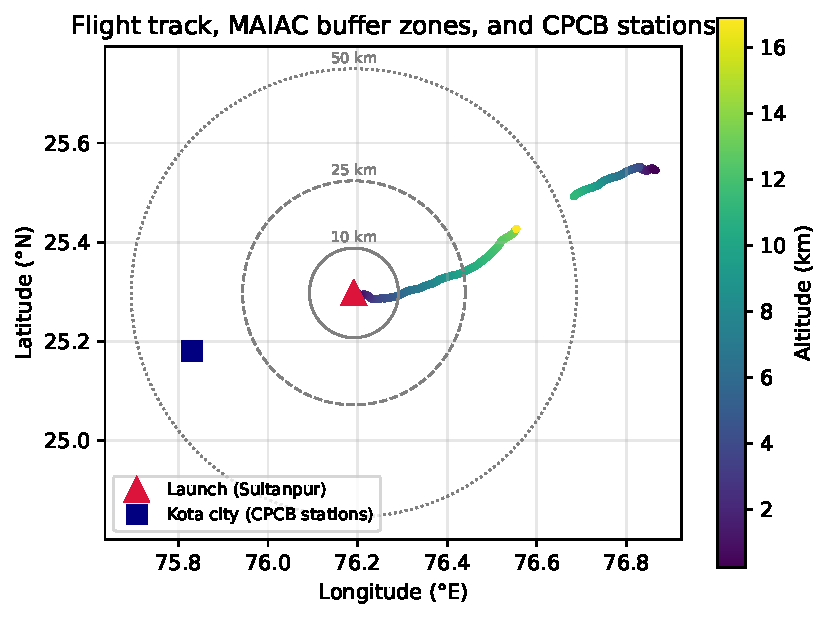
\includegraphics[width=0.62\textwidth]{F6_map.pdf}
\caption{Flight track coloured by altitude, with the 10/25/50-km MAIAC AOD buffer zones
around the Sultanpur launch site (triangle) and the location of Kota city with its two
CPCB monitoring stations (square).}
\label{fig:f6}
\end{figure}

\subsection{Payload}

Table~\ref{tab:payload} summarises the payload. The primary instrument is an Apogee SU-202
amplified UV-A radiometer: spectral range 305--390~nm, output 0--2.5~V over
0--100~W\,m$^{-2}$ (calibration factor 0.04~W\,m$^{-2}$\,mV$^{-1}$), calibration
uncertainty $\pm$5\%, repeatability $<$0.5\%, non-linearity $<$1\%, temperature response
$<$0.1\%\,$^\circ$C$^{-1}$, directional (cosine) error $\pm$2\% at 45$^\circ$ and
$\pm$5\% at 75$^\circ$, operating range $-40$ to $+70^\circ$C \cite{apogee}. The remaining
channels provide context and are treated as secondary.

\begin{table}[htbp]
\centering
\footnotesize
\caption{Payload channels, roles, and status during the flight.}
\label{tab:payload}
\begin{tabular}{llll}
\toprule
Channel & Instrument class & Role & Status \\
\midrule
UV-A irradiance & Apogee SU-202 radiometer & \textbf{Primary} & nominal throughout \\
$P$, $T$, RH & BME280-class combined sensor & altitude, met & nominal ($T$ payload-internal) \\
Ionising counts & GM counter (CPM) & cosmic-ray context & valid $<$4.7~km; HV failure \\
O$_3$ & semiconductor gas sensor & context & non-responsive (0.00) \\
GPS & u-blox-class receiver & position, time & position ok; time froze \\
Video camera + IMU & Runcam camera, 1-kHz gyro/accel & attitude, documentation & nominal throughout \\
Thermal imager & IR pixel array & qualitative & not analysed here \\
\bottomrule
\end{tabular}
\end{table}

\subsection{Timekeeping correction}

GPS time-stamps froze intermittently at altitude (a known behaviour of consumer GPS
modules on HAB flights), while the logger's real-time clock (RTC) ticked steadily. All
times used here are RTC times anchored to the first valid GPS fix (IST). Solar position
was computed per sample with the NOAA solar geometry algorithm using GPS coordinates.
The timeline is independently corroborated by the onboard camera's 1-kHz IMU log, in
which the release jerk, the balloon-burst onset of violent rotation, and the 18.6-$g$
landing impact appear with relative spacings that match the RTC timeline to within
$\approx$1~minute.

\subsection{Payload attitude from the camera IMU}

The action camera recorded continuous 1-kHz gyroscope and accelerometer logs (GyroFlow
format) for the whole flight, providing a free, quantitative record of payload attitude.
During ascent the payload rotated slowly about the suspension axis (median angular rate
0.72~rad\,s$^{-1}$, $\approx$6.8~rpm) and swung very little: the tilt of the low-passed
gravity vector from its slow mean had a median of 0.9$^\circ$, a 95th percentile of
2.6$^\circ$, and a 99th percentile of 3.9$^\circ$. Because the payload completes roughly
18 rotations within each 500-m altitude bin, the first-order (azimuth-dependent) cosine
error of a tilted sensor averages toward zero, and the residual swing noise appears in
the within-bin scatter that the uncertainty budget already propagates
(Section~3). The tilt allowance used below is therefore grounded in measurement rather
than assumption. Descent under parachute was rougher (median tilt 1.4$^\circ$, 95th
percentile 5.6$^\circ$), one more reason descent data are excluded from the retrieval.

\subsection{Ancillary public data}

Four public datasets from the flight day provide context: (i)~MAIAC MCD19A2 AOD at 470 and
550~nm \cite{lyapustin2018}, extracted along the flight track (0.781 and 0.610
respectively) and in buffers of 10--100~km around the launch site; (ii)~Sentinel-5P TROPOMI
\cite{veefkind2012} column products along the track (O$_3$ 281~DU; NO$_2$
23~$\mu$mol\,m$^{-2}$; SO$_2$ 0.21~mmol\,m$^{-2}$; CO 0.029~mol\,m$^{-2}$; UV aerosol index
$-0.19$); (iii)~ERA5 reanalysis \cite{hersbach2020} (boundary-layer height 1{,}411~m,
cloud-base height 1{,}290~m, 2-m temperature 306.4~K); (iv)~CPCB continuous
ambient air-quality data from the two Kota stations (Nayapura; Shrinath Puram), reporting
4-hourly PM$_{2.5}$, PM$_{10}$, NO$_2$, NH$_3$, CO and SO$_2$ \cite{cpcb}; and (v)~the
NASA POWER SYN1DEG-based hourly surface UV-A product at the launch coordinates
\cite{power}, used as an independent cross-check of the radiometer.

\section{Uncertainty budget and error propagation}

\subsection{Per-sample irradiance}

Irradiance is $E = cV$ with $c = 40$~W\,m$^{-2}$\,V$^{-1}$. Uncertainty terms combine in
quadrature:
\begin{equation}
\frac{\sigma_E}{E} \;=\;
\sqrt{u_{\mathrm{cal}}^2 + u_{\mathrm{lin}}^2 + u_{\mathrm{rep}}^2
      + u_{\cos}^2 + \big(u_T\,|T-25|\big)^2
      + \Big(\tfrac{\sigma_q}{V}\Big)^2},
\label{eq:esig}
\end{equation}
with $u_{\mathrm{cal}}=5\%$, $u_{\mathrm{lin}}=1\%$, $u_{\mathrm{rep}}=0.5\%$,
$u_{\cos}=2\%$ (5\% for SZA $>72^\circ$), $u_T=0.1\%\,^\circ$C$^{-1}$, and quantisation
$\sigma_q = 0.01/\sqrt{12}$~V from the logged resolution. Over the flight the median total
uncertainty is $\pm$5.8\% ($k$=1; worst case 9.1\% at the low-signal launch condition), of
which only 2.1\% is random (Table~\ref{tab:budget}).

\begin{table}[htbp]
\centering
\footnotesize
\caption{Error budget for UV-A irradiance and derived quantities.}
\label{tab:budget}
\begin{tabular}{llll}
\toprule
Term & Magnitude & Type & Enters $\tau_{\mathrm{eff}}$? \\
\midrule
Calibration & $\pm$5\% & systematic & cancels in ratio \\
Non-linearity & $\pm$1\% & systematic & cancels (1st order) \\
Repeatability & $\pm$0.5\% & random & yes \\
Cosine/tilt & $\pm$2\% ($\pm$5\% SZA$>72^\circ$); tilt p95 2.6$^\circ$ & random (swing) & yes \\
Temperature response & $\le$0.1\%\,$^\circ$C$^{-1}\times|T-25|$ & systematic & partially \\
Quantisation (0.01~V) & 0.15--7\% & random & yes \\
\midrule
Altitude (BME280, $\pm$1~hPa) & $\pm$8.7~m (surface) to $\pm$96~m (apogee) & systematic & negligible (500-m bins) \\
GM counting & Poisson $\sqrt{N}$ & random & --- \\
\bottomrule
\end{tabular}
\end{table}

\subsection{Effective optical depth}

Samples are averaged in 500-m altitude bins (ascent only). Modelling global irradiance
with a Beer--Lambert form,
\begin{equation}
\ln E \;=\; \ln E_0 + \ln\cos\theta_s \;-\; m(\theta_s)\,\tau_{\mathrm{eff}}(z),
\label{eq:langley}
\end{equation}
where $m(\theta_s)$ is the Kasten--Young relative air mass \cite{kasten1989} and
$\tau_{\mathrm{eff}}(z)$ is the \emph{effective} vertical optical depth of the column above
altitude $z$, we anchor the retrieval at apogee with
$\tau_{\mathrm{eff}}(z_{\mathrm{apo}}) = \tau_R(360)\,P_{\mathrm{apo}}/P_0 + 0.005 = 0.050$
(residual Rayleigh above 81~hPa plus stratospheric aerosol). The Rayleigh optical depth
uses $\tau_R(\lambda) = 0.0088\,\lambda^{-4.05}\,P/P_0$ ($\lambda$ in $\mu$m)
\cite{bodhaine1999}, giving $\tau_R = 0.551$ at the sensor's effective wavelength
($\approx$360~nm). Because the anchor and every sample share the same calibration factor,
the $\pm$5\% calibration and non-linearity terms cancel in
Eq.~(\ref{eq:langley}); the propagated uncertainty of $\tau_{\mathrm{eff}}$ retains only
the random terms of the two bins involved:
\begin{equation}
\sigma_{\tau}(z) \;=\; \frac{1}{m(\theta_s)}
\sqrt{\sigma_{\ln E}^2(z) + \sigma_{\ln E}^2(z_{\mathrm{apo}})}.
\end{equation}
The implied extraterrestrial constant, $E_0 = 102$~W\,m$^{-2}$, is $\sim$20\% above the
nominal top-of-atmosphere UV-A irradiance for this band ($\approx$85~W\,m$^{-2}$),
consistent with the combined calibration, spectral-band and tilt systematics discussed in
Section~\ref{sec:limits}; this offset does not affect $\tau_{\mathrm{eff}}$.

\subsection{Satellite comparison quantities}

The \r{A}ngstr\"om exponent \cite{angstrom1929} from the along-track MAIAC pair is
$\alpha = \ln(0.781/0.610)/\ln(550/470) = 1.57$, giving
$\mathrm{AOD}_{360} = 0.610\,(550/360)^{1.57} = 1.19 \pm 0.21$, where the uncertainty
combines the MAIAC expected error over land ($\pm 0.05 \pm 0.1\,\mathrm{AOD}$) and a 10\%
extrapolation allowance. The direct-beam extinction expectation is then
$\tau_{\mathrm{ext}} = \tau_R + \mathrm{AOD}_{360} = 1.74 \pm 0.21$.

\section{Results}

\subsection{Profiles}

Figure~\ref{fig:f1} shows the flight profile and payload-internal thermodynamic record.
Figure~\ref{fig:f2}a shows measured UV-A irradiance increasing from 7.6 to
79.2~W\,m$^{-2}$ between the surface and apogee. Most of that increase is solar geometry:
after normalising by $\cos\theta_s$ (Fig.~\ref{fig:f2}b) the profile is nearly constant
above $\approx$3~km and drops only in the lowest 2--3~km, where the aerosol column
resides.

\begin{figure}[htbp]
\centering
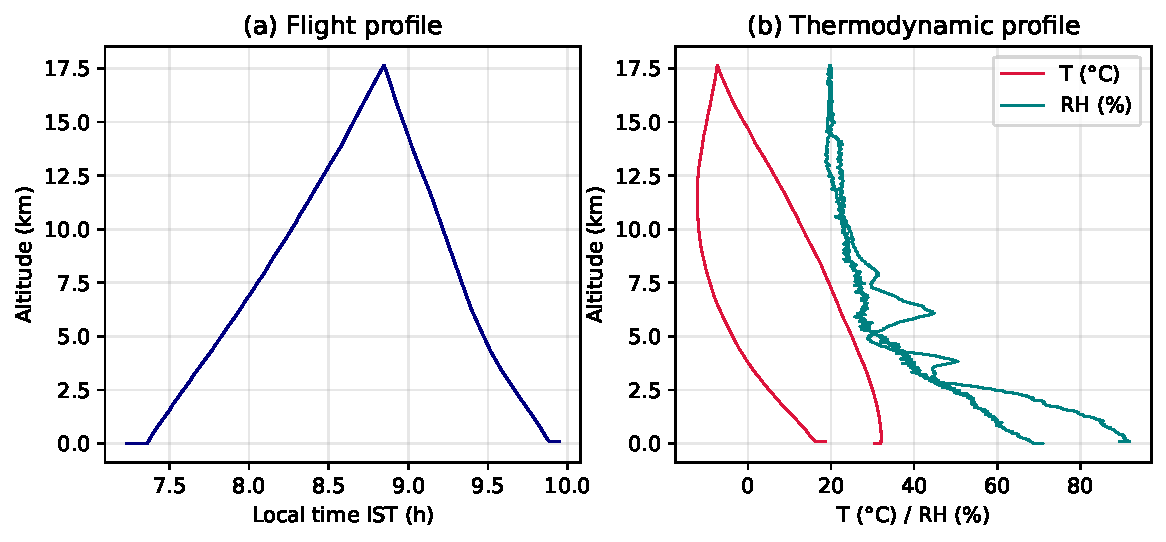
\includegraphics[width=0.95\textwidth]{F1_overview.pdf}
\caption{(a) Altitude--time record (RTC-anchored IST). (b) Payload-internal temperature
and relative-humidity profiles.}
\label{fig:f1}
\end{figure}

\begin{figure}[htbp]
\centering
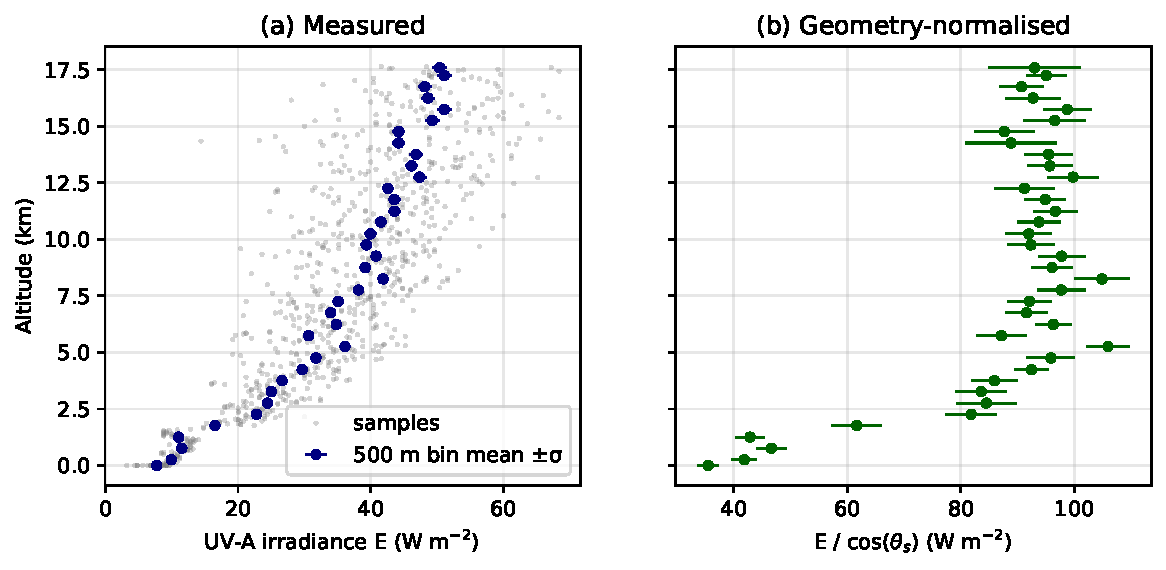
\includegraphics[width=0.95\textwidth]{F2_uv_profile.pdf}
\caption{(a) Global UV-A irradiance vs.\ altitude: individual 7-s samples (grey) and
500-m bin means with $\pm 1\sigma$ random uncertainty (blue). (b) The same bins normalised
by $\cos\theta_s$; the residual altitude dependence below $\approx$3~km is atmospheric
attenuation.}
\label{fig:f2}
\end{figure}

\subsection{Effective optical depth of global UV-A}

The Langley-anchored retrieval (Fig.~\ref{fig:f3}) yields a surface value
\begin{equation*}
\tau_{\mathrm{eff}} = 0.233 \pm 0.023 ,
\end{equation*}
i.e.\ a vertical-equivalent transmittance of global UV-A of
$e^{-\tau_{\mathrm{eff}}} = 0.79$. Roughly 90\% of the column effect accumulates below
$\approx$2.5~km, with the sharpest decrease in the 1.5--2.5~km layer --- at and just above
the ERA5 boundary-layer top (1.41~km) and cloud base (1.29~km) --- consistent with aerosol
and scattered cloud accumulating at the top of the shallow morning boundary layer. The
lowest bins were measured at SZA~$>72^\circ$ and constrain the sub-1.5-km contribution
only weakly.

\begin{figure}[htbp]
\centering
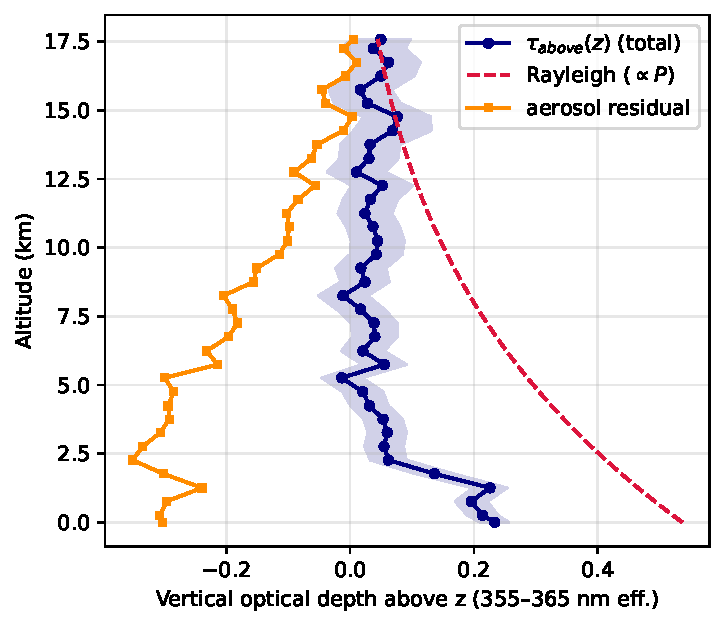
\includegraphics[width=0.62\textwidth]{F3_tau_profile.pdf}
\caption{Effective vertical optical depth above altitude $z$ for global UV-A (blue, with
$\pm1\sigma$ envelope), the Rayleigh extinction profile (dashed), and their difference
(orange). $\tau_{\mathrm{eff}}$ falling \emph{below} the Rayleigh extinction curve is the
signature of diffuse replenishment: scattering removes photons from the direct beam but
returns most of them to the downwelling hemisphere, which is what a 180$^\circ$
field-of-view radiometer measures.}
\label{fig:f3}
\end{figure}

\subsection{Global vs.\ direct-beam attenuation}

Figure~\ref{fig:f4} compares the measured $\tau_{\mathrm{eff}}$ with the direct-beam
expectation. The ratio
\begin{equation*}
\eta \;=\; \frac{\tau_{\mathrm{eff}}}{\tau_{\mathrm{ext}}} \;=\; 0.134 \pm 0.021
\end{equation*}
states that the real atmosphere on this day attenuated hemispherical UV-A only
$\approx$13\% as strongly as it attenuated the direct beam. Two independent observations
support the interpretation that scattering (not absorption) dominated the extinction:
the TROPOMI UV aerosol index was slightly negative ($-0.19$, non-absorbing), and surface
PM$_{2.5}$ was moderate (24--29~$\mu$g\,m$^{-3}$). For a purely scattering,
high-single-scattering-albedo column, most extinguished direct-beam photons reappear as
diffuse sky radiance, so $\eta \ll 1$ is the physically expected regime; $\eta$ would
approach unity only for a strongly absorbing column.

\begin{figure}[htbp]
\centering
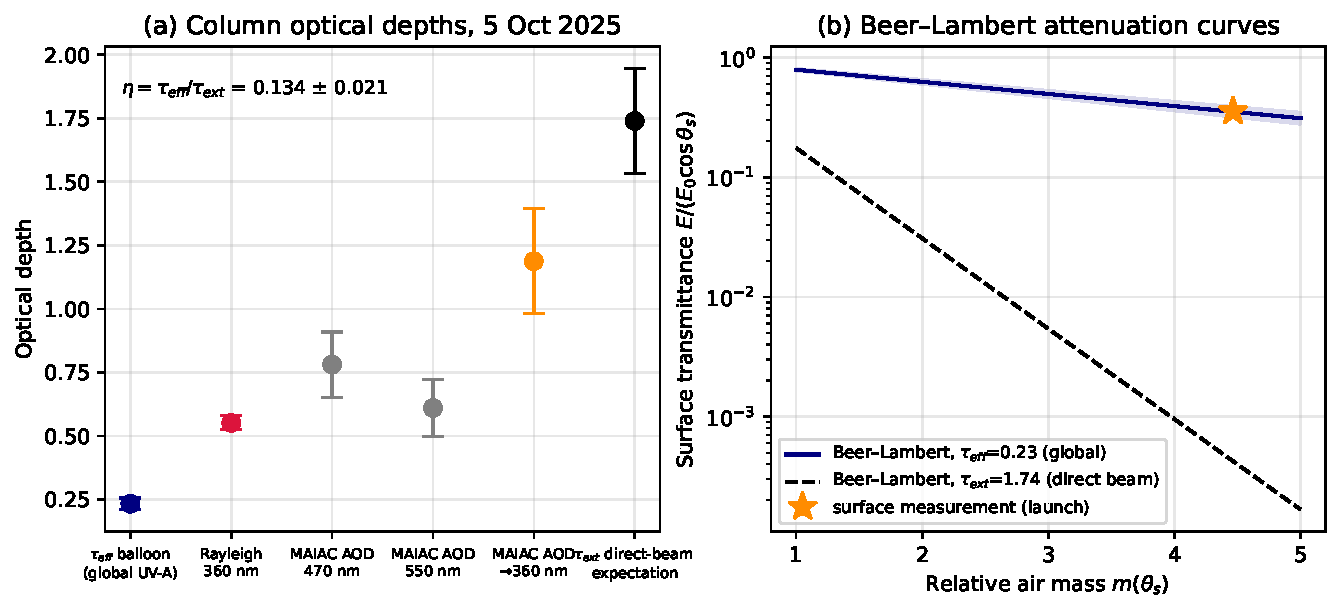
\includegraphics[width=0.98\textwidth]{F4_closure.pdf}
\caption{(a) Optical-depth comparison for 5~October~2025 over the Kota region. Blue:
balloon-derived effective optical depth for global UV-A. Red: Rayleigh extinction at
360~nm. Grey: MAIAC along-track AOD at 470 and 550~nm. Orange: MAIAC AOD extrapolated to
360~nm with $\alpha = 1.57$. Black: direct-beam extinction expectation (Rayleigh +
aerosol). (b) The same result as Beer--Lambert attenuation curves: surface transmittance
vs.\ air mass for the measured effective optical depth (solid, with $\pm1\sigma$ band) and
for the direct-beam expectation (dashed). The pre-launch surface measurement (star) lies
on the global-irradiance curve; the direct-beam curve at that air mass predicts a
transmittance $\approx$900$\times$ smaller, which is the clearest visual statement that a
hemispherical sensor under a scattering atmosphere is dominated by diffuse irradiance.}
\label{fig:f4}
\end{figure}

\subsection{Spatial representativeness of the satellite AOD}

MAIAC 550-nm AOD statistics in growing buffers around the launch site show a systematic
dilution with distance: mean 0.664 ($\pm$0.038) within 10~km, 0.635 ($\pm$0.103) within
25~km, 0.554 ($\pm$0.125) within 50~km, and 0.461 ($\pm$0.102) within 100~km. The
along-track value (0.610) sits between the 10 and 25~km buffer means, indicating the
flight sampled air representative of the urban core rather than the cleaner surroundings
--- a scale effect consistent with validation practice for satellite AOD
\cite{payra2023,attey2025}.

\subsection{Context: surface air quality and cosmic-ray counts}

Figure~\ref{fig:f5}a places the flight within the CPCB record: daily-mean PM$_{2.5}$ on
launch day was 24.2~$\mu$g\,m$^{-3}$ (Nayapura) and 28.6~$\mu$g\,m$^{-3}$ (Shrinath
Puram), with 31.6 and 28.2~$\mu$g\,m$^{-3}$ in the 08:00--12:00 window --- a moderate
pollution day, well below the post-Diwali November peaks visible later in the same record.
The GM channel (Fig.~\ref{fig:f5}b) shows the expected secondary cosmic-ray increase from
30~CPM at the surface to a median 72~CPM at 4--4.5~km ($\times$2.4, Poisson
$\sigma=\sqrt{N}$), before failing above 4.7~km (Section~\ref{sec:lessons}).

\begin{figure}[htbp]
\centering
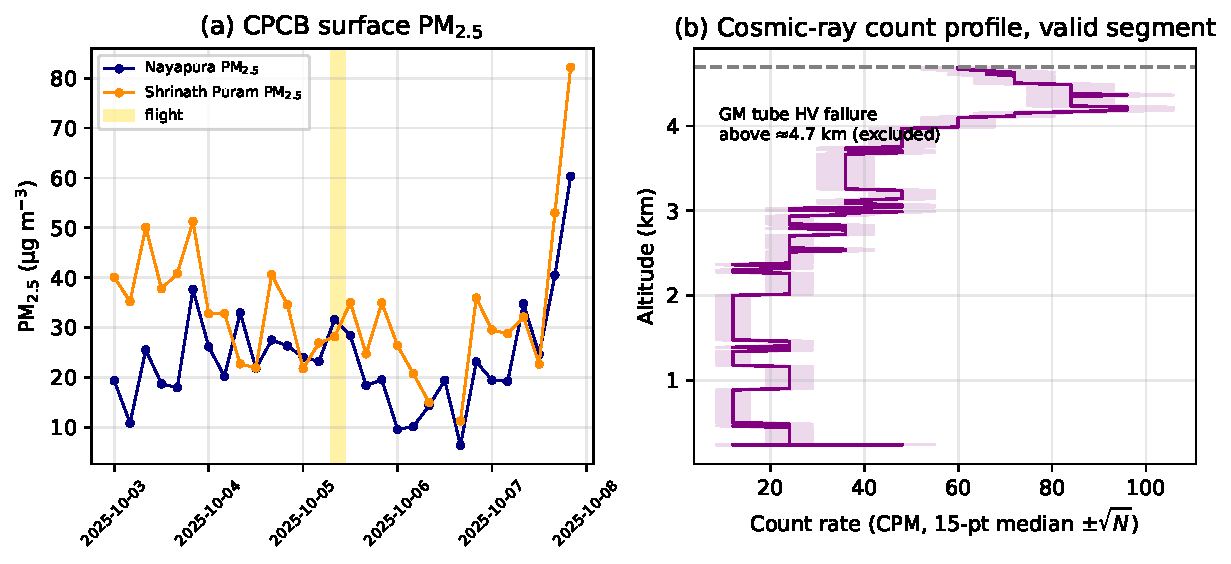
\includegraphics[width=0.95\textwidth]{F5_context.pdf}
\caption{(a) CPCB 4-hourly PM$_{2.5}$ at the two Kota stations, 3--8 October 2025; the
gold band marks the flight. (b) GM count-rate profile over the valid segment
(15-point median $\pm\sqrt{N}$); data above the high-voltage failure at $\approx$4.7~km
are excluded.}
\label{fig:f5}
\end{figure}

\subsection{Independent surface cross-check against NASA POWER}

The radiometer can be referenced against an independent, satellite-derived estimate of
surface UV-A. The NASA POWER hourly product (SYN1DEG; 1$^\circ$ resolution, 315--400~nm
band) for the launch coordinates gives, interpolated to the pre-launch epoch
(07:19~IST), 6.5~W\,m$^{-2}$; the level, ground-based SU-202 read 8.0~W\,m$^{-2}$ ---
agreement within $\approx$25\%, which is consistent with the combined effect of the
1$^\circ$ footprint, the steep sunrise ramp within the product's hourly averaging window,
the slight band mismatch (315--400 vs.\ 305--390~nm), and the sensor's low-signal
quantisation at that hour. After touchdown (09:54~IST) the sensor read 11.7~W\,m$^{-2}$
against a POWER value of 35.6~W\,m$^{-2}$: the landed payload no longer viewed the full
sky, and all post-touchdown data are accordingly excluded from analysis --- a reminder
that orientation control ends at landing, not at descent.

\section{Instrument lessons}
\label{sec:lessons}

Three failures on this flight are instructive for HAB payload design and are reported so
that others can avoid them:

\begin{enumerate}
\item \textbf{GM-tube corona discharge at low pressure.} Above $\approx$4.7~km
(P $\lesssim$ 550~hPa) the count rate jumped from $\sim$10$^2$ to $>$10$^5$~CPM and then
fell to zero: the high-voltage supply arced in thin air. Counts above 4.7~km were
discarded. Conformal coating or a sealed tube enclosure is recommended.
\item \textbf{Non-responsive O$_3$ channel.} The semiconductor ozone sensor read 0.00
throughout; heater-type metal-oxide gas sensors need minutes of warm-up power and ambient
temperatures they never see on ascent. Electrochemical cells or pre-heated enclosures are
preferable.
\item \textbf{GPS time-stamp freezing.} Position remained usable but time strings froze
intermittently at altitude. Anchoring the RTC to the first valid GPS fix recovered a
reliable timeline (verified by a physical 3.0~m\,s$^{-1}$ mean ascent rate and by the
IMU event chain); logging both clocks is essential because solar-geometry corrections are
only as good as the timeline.
\end{enumerate}

One positive lesson balances the three failures: an ordinary action camera with gyro
logging (intended for video stabilisation) doubles as a free 1-kHz attitude sensor. It
quantified payload tilt and rotation, independently confirmed the event timeline, and
documented sky conditions --- capabilities that would otherwise require a dedicated IMU
payload. We recommend gyro-logging cameras as standard equipment on radiometric HAB
flights.

\section{Limitations}
\label{sec:limits}

This is a single flight with a hemispherical broadband sensor, and four caveats bound the
interpretation. (i)~$\tau_{\mathrm{eff}}$ is an \emph{effective} (global-irradiance)
quantity, not extinction AOD; the Beer--Lambert form of Eq.~(\ref{eq:langley}) is an
operational definition, and the plane-parallel air-mass treatment of the diffuse component
is approximate, particularly at the large launch SZA. Moreover, the morning was partly
cloudy below $\approx$3~km, so $\tau_{\mathrm{eff}}$ is an all-sky effective quantity
while the MAIAC AOD it is compared against is cloud-screened; part of the
boundary-layer-concentrated attenuation may be broken-cloud rather than aerosol
extinction. (ii)~Payload tilt under balloon swing is now measured (median 0.9$^\circ$,
95th percentile 2.6$^\circ$, with $\approx$6.8~rpm rotation averaging the first-order
cosine error), so this term is bounded rather than assumed. (iii)~The effective wavelength
of the 305--390~nm band ($\approx$360~nm) carries uncertainty that maps onto $\tau_R$ and
the \r{A}ngstr\"om extrapolation. (iv)~The implied $E_0$ exceeds the nominal
top-of-atmosphere value by $\sim$20\%, indicating residual absolute-scale systematics
(calibration transfer, spectral response, tilt); ratio-based quantities
($\tau_{\mathrm{eff}}$, $\eta$) are insensitive to this scale. A repeat flight near local
noon, a shaded/global sensor pair, or an added narrowband photodiode would separate the
direct and diffuse components directly.

\section{Conclusions}

A low-cost HAB flight with one research-grade radiometer and rigorous error propagation
produced a quantitative, uncertainty-bounded result: on a moderately turbid, non-absorbing
day over Kota, the vertical effective optical depth of global UV-A was
$0.233 \pm 0.023$ --- only $13.4 \pm 2.1$\% of the direct-beam extinction expectation
constructed from Rayleigh theory and satellite AOD. The attenuation was concentrated below
$\approx$2.5~km, chiefly in the layer at and just above the reanalysis boundary-layer top
and cloud base. The flight also
demonstrated, through three documented failures, where student-class payloads are fragile.
The combination of a calibrated primary sensor, cancellation-aware uncertainty analysis,
and free public satellite/reanalysis/regulatory data is reproducible by any school or
university group, and repeat flights across seasons would turn this case study into a
useful climatology of UV attenuation for the region.

\section*{Data and code availability}
The flight datalog, cleaned profiles, analysis scripts, and figure-generation code are
available at \url{https://github.com/1boscochiramel/AkashaJyoti-UVA-Kota}.

\section*{Acknowledgments}
The author thanks Mani Joe for contributions to payload preparation and data processing,
and Archana Radhakrishnan for contributions to mission planning and data interpretation,
during the earlier phase of the project. The author also thanks Rohit Kulkarni for
payload integration; Yashashwi Chaudhary for enclosure design; Tanuja Pant for
flight-termination system design; Aaruhi for regulatory coordination support; Ahan Ray
for procurement; and Hem Prasath and Shree Ranganathan for mission operations and launch
logistics. The public datasets used here are operated by NASA (MAIAC MCD19A2; POWER),
ESA/Copernicus (Sentinel-5P TROPOMI; ERA5 via CDS), and the Central Pollution Control
Board of India.

\section*{Conflicts of interest}
The author declares no conflicts of interest.

\begin{thebibliography}{99}\small

\bibitem{malings2020} Malings, C., et al. (2020). Application of low-cost fine particulate
mass monitors to convert satellite aerosol optical depth to surface concentrations in
North America and Africa. \emph{Atmospheric Measurement Techniques}, 13, 3873--3892.

\bibitem{lin2020} Lin, C., et al. (2020). Observation of PM$_{2.5}$ using a combination of
satellite remote sensing and low-cost sensor network in Siberian urban areas with limited
reference monitoring. \emph{Atmospheric Environment}, 227, 117410.

\bibitem{attey2025} Attey-Yeboah, P., et al. (2025). Utility of low-cost sensor
measurement for predicting ambient PM$_{2.5}$ concentrations: evidence from a monitoring
network in Accra, Ghana. \emph{Environmental Science: Atmospheres}, 5, 517--530.

\bibitem{dey2020} Dey, S., et al. (2020). A satellite-based high-resolution (1-km) ambient
PM$_{2.5}$ database for India over two decades (2000--2019). \emph{Remote Sensing}, 12, 2773.

\bibitem{maheshwarkar2021} Maheshwarkar, P., et al. (2021). Population exposure across
central India to PM$_{2.5}$ derived using remotely sensed products in a three-stage
statistical model. \emph{Scientific Reports}, 11, 544.

\bibitem{payra2023} Payra, S., et al. (2023). Performance evaluation of MODIS and VIIRS
satellite AOD products over the Indian subcontinent. \emph{Frontiers in Environmental
Science}, 11.

\bibitem{renard2020} Renard, J.-B., et al. (2020). Vertical profiles of pollution particle
concentrations in the boundary layer above Paris (France) from the optical aerosol counter
LOAC onboard a touristic balloon. \emph{Sensors}, 20(4), 1111.

\bibitem{brattich2019} Brattich, E., et al. (2019). Measurements of aerosols and charged
particles on the BEXUS18 stratospheric balloon. \emph{Annales Geophysicae}, 37, 389--403.

\bibitem{potosnak2021} Potosnak, M., et al. (2021). Tropospheric sounding with low-cost
particulate matter sensors. \emph{Journal of High Altitude Ballooning}, 1(1).

\bibitem{pang2020} Pang, X., et al. (2020). A lightweight low-cost and multipollutant
sensor package for aerial observations of air pollutants in atmospheric boundary layer.
\emph{Science of the Total Environment}, 764, 142828.

\bibitem{molina2023} Molina Rueda, E., et al. (2023). Size-resolved field performance of
low-cost sensors for particulate matter air pollution. \emph{Environmental Science \&
Technology Letters}, 10(3), 247--253.

\bibitem{giordano2021} Giordano, M. R., et al. (2021). From low-cost sensors to
high-quality data: A summary of challenges and best practices for effectively calibrating
low-cost particulate matter mass sensors. \emph{Journal of Aerosol Science}, 158, 105833.

\bibitem{kasten1989} Kasten, F., \& Young, A. T. (1989). Revised optical air mass tables
and approximation formula. \emph{Applied Optics}, 28(22), 4735--4738.

\bibitem{bodhaine1999} Bodhaine, B. A., Wood, N. B., Dutton, E. G., \& Slusser, J. R.
(1999). On Rayleigh optical depth calculations. \emph{Journal of Atmospheric and Oceanic
Technology}, 16(11), 1854--1861.

\bibitem{angstrom1929} \r{A}ngstr\"om, A. (1929). On the atmospheric transmission of sun
radiation and on dust in the air. \emph{Geografiska Annaler}, 11(2), 156--166.

\bibitem{lyapustin2018} Lyapustin, A., Wang, Y., Korkin, S., \& Huang, D. (2018). MODIS
Collection 6 MAIAC algorithm. \emph{Atmospheric Measurement Techniques}, 11, 5741--5765.

\bibitem{veefkind2012} Veefkind, J. P., et al. (2012). TROPOMI on the ESA Sentinel-5
Precursor: A GMES mission for global observations of the atmospheric composition for
climate, air quality and ozone layer applications. \emph{Remote Sensing of Environment},
120, 70--83.

\bibitem{hersbach2020} Hersbach, H., et al. (2020). The ERA5 global reanalysis.
\emph{Quarterly Journal of the Royal Meteorological Society}, 146(730), 1999--2049.

\bibitem{apogee} Apogee Instruments (2024). \emph{SU-200 series UV sensors --- owner's
manual and specifications}. Logan, UT, USA. \url{https://www.apogeeinstruments.com}.

\bibitem{power} NASA Langley Research Center (2025). \emph{POWER: Prediction Of Worldwide
Energy Resources --- hourly time series (SYN1DEG)}. \url{https://power.larc.nasa.gov}.

\bibitem{cpcb} Central Pollution Control Board (2025). \emph{Continuous Ambient Air
Quality Monitoring System (CAAQMS) data portal}. New Delhi, India.
\url{https://airquality.cpcb.gov.in}.

\end{thebibliography}

\end{document}
